\documentclass[12pt]{report}\usepackage[]{graphicx}\usepackage[dvipsnames]{xcolor}
% maxwidth is the original width if it is less than linewidth
% otherwise use linewidth (to make sure the graphics do not exceed the margin)
\makeatletter
\def\maxwidth{ %
  \ifdim\Gin@nat@width>\linewidth
    \linewidth
  \else
    \Gin@nat@width
  \fi
}
\makeatother

\definecolor{fgcolor}{rgb}{0.345, 0.345, 0.345}
\newcommand{\hlnum}[1]{\textcolor[rgb]{0.686,0.059,0.569}{#1}}%
\newcommand{\hlstr}[1]{\textcolor[rgb]{0.192,0.494,0.8}{#1}}%
\newcommand{\hlcom}[1]{\textcolor[rgb]{0.678,0.584,0.686}{\textit{#1}}}%
\newcommand{\hlopt}[1]{\textcolor[rgb]{0,0,0}{#1}}%
\newcommand{\hlstd}[1]{\textcolor[rgb]{0.345,0.345,0.345}{#1}}%
\newcommand{\hlkwa}[1]{\textcolor[rgb]{0.161,0.373,0.58}{\textbf{#1}}}%
\newcommand{\hlkwb}[1]{\textcolor[rgb]{0.69,0.353,0.396}{#1}}%
\newcommand{\hlkwc}[1]{\textcolor[rgb]{0.333,0.667,0.333}{#1}}%
\newcommand{\hlkwd}[1]{\textcolor[rgb]{0.737,0.353,0.396}{\textbf{#1}}}%
\let\hlipl\hlkwb

\usepackage{framed}
\makeatletter
\newenvironment{kframe}{%
 \def\at@end@of@kframe{}%
 \ifinner\ifhmode%
  \def\at@end@of@kframe{\end{minipage}}%
  \begin{minipage}{\columnwidth}%
 \fi\fi%
 \def\FrameCommand##1{\hskip\@totalleftmargin \hskip-\fboxsep
 \colorbox{shadecolor}{##1}\hskip-\fboxsep
     % There is no \\@totalrightmargin, so:
     \hskip-\linewidth \hskip-\@totalleftmargin \hskip\columnwidth}%
 \MakeFramed {\advance\hsize-\width
   \@totalleftmargin\z@ \linewidth\hsize
   \@setminipage}}%
 {\par\unskip\endMakeFramed%
 \at@end@of@kframe}
\makeatother

\definecolor{shadecolor}{rgb}{.97, .97, .97}
\definecolor{messagecolor}{rgb}{0, 0, 0}
\definecolor{warningcolor}{rgb}{1, 0, 1}
\definecolor{errorcolor}{rgb}{1, 0, 0}
\newenvironment{knitrout}{}{} % an empty environment to be redefined in TeX

\usepackage{alltt}

\usepackage[utf8]{inputenc}
\usepackage[spanish]{babel}
\usepackage[margin=2.54cm]{geometry}
\usepackage[dvipsnames]{xcolor}
\usepackage{array, amssymb, amsthm, enumitem, fancyhdr, float, graphicx, hyperref, hologo, mathtools, tikz, tikz-cd}
\usepackage[spanish, noabbrev]{cleveref}

\pagestyle{fancy}
\lhead{\footnotesize \leftmark}
\rhead{\footnotesize \rightmark}

\title{
	\huge
	\noindent\textbf{Fundamentos de la Ciencia de Datos}\\
	
	{\Large \textit{Práctica 1}}
	\vspace{1cm}
	
	\huge
	Grado en Ingeniería Informática\\
	Universidad de Alcalá\\
	
	\vspace{1cm}
	
	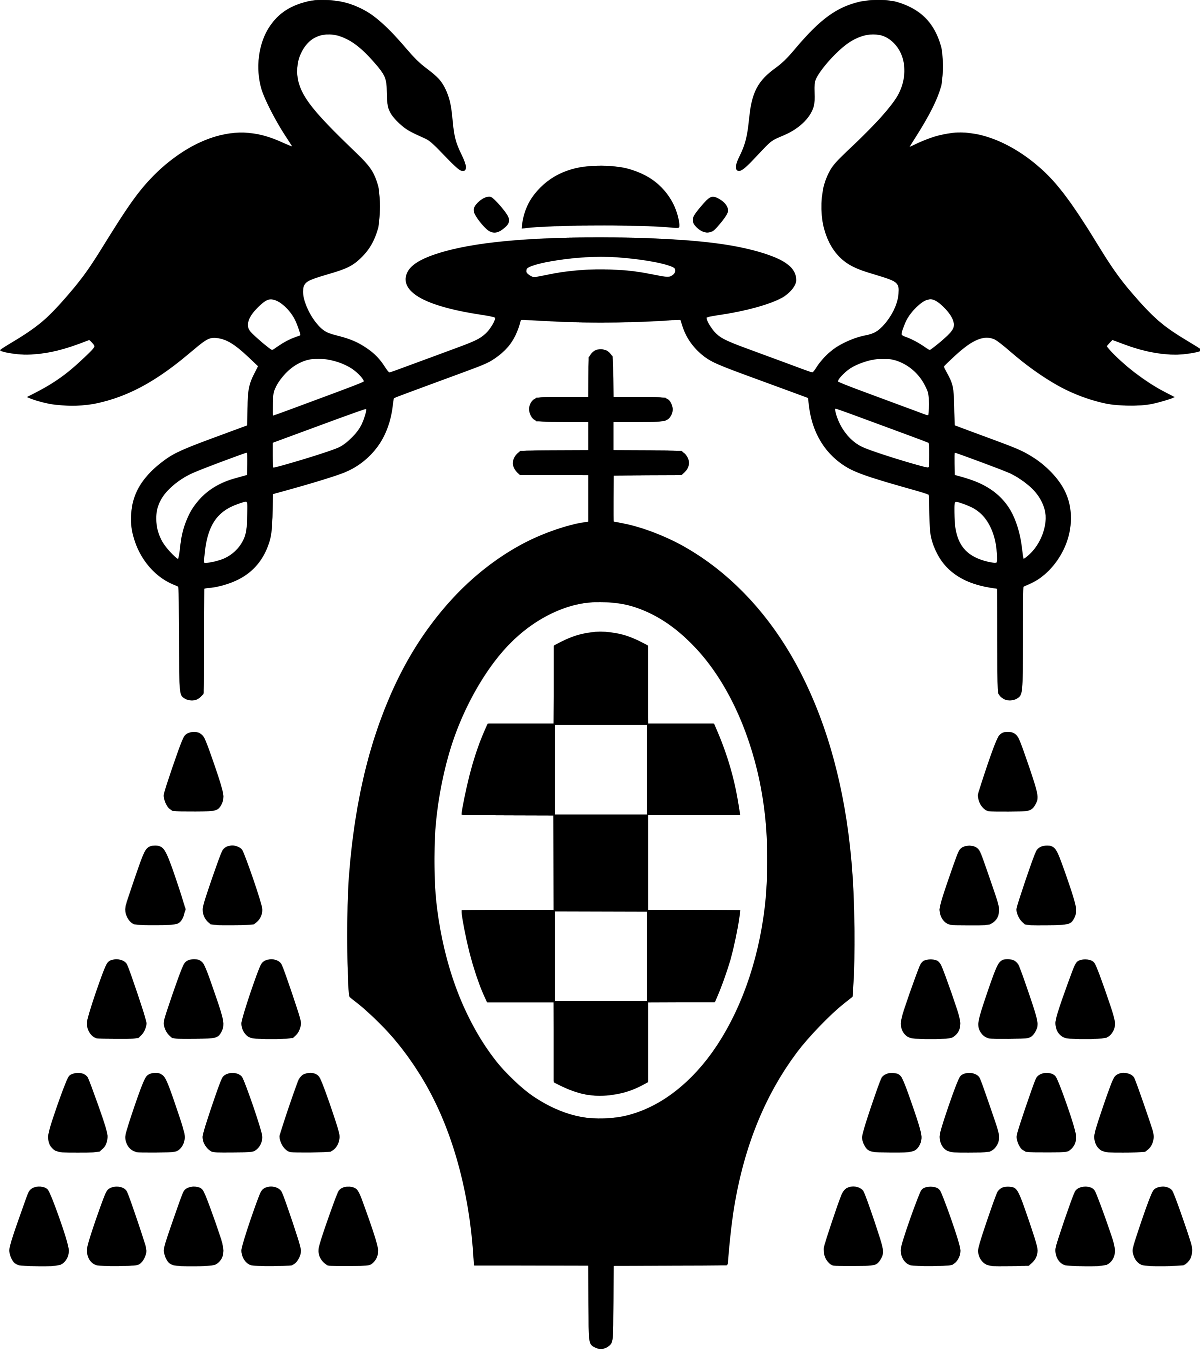
\includegraphics[scale=0.075]{img/logo}
}

\author{
	Pablo García García\\
	Abel López Martínez\\
	Álvaro Jesús Martínez Parra\\
	Raúl Moratilla Núñez
}

\date{
	\large{14 de noviembre de 2023}
}

\hypersetup{
	pdftitle={Práctica 1}, 
	pdfauthor={Pablo García García, Abel López Martínez, Álvaro Jesús Martínez Parra, Raúl Moratilla Núñez}, 
	pdfsubject={Fundamentos de la Ciencia de Datos}, 
	pdfcenterwindow, 
	pdfnewwindow=true, 
	pdfkeywords={Entrega de la PL1 de laboratorio correspondiente al Curso 2023-2024}, 
	bookmarksopen=true 
}
\IfFileExists{upquote.sty}{\usepackage{upquote}}{}
\begin{document}
	
\begin{knitrout}
\definecolor{shadecolor}{rgb}{0.969, 0.969, 0.969}\color{fgcolor}\begin{kframe}
\begin{alltt}
\hlstd{fichero} \hlkwb{=} \hlkwd{read.csv2}\hlstd{(}\hlstr{"distancia_universitarios.csv"}\hlstd{)}

\hlstd{len} \hlkwb{=} \hlkwa{function}\hlstd{(}\hlkwc{list}\hlstd{)\{}
        \hlstd{count} \hlkwb{=} \hlnum{0}
        \hlkwa{for} \hlstd{(element} \hlkwa{in} \hlstd{list)\{}
                \hlstd{count} \hlkwb{=} \hlstd{count} \hlopt{+} \hlnum{1}
        \hlstd{\}}
        \hlstd{count}
\hlstd{\}}

\hlstd{distancias} \hlkwb{=} \hlstd{fichero}\hlopt{$}\hlstd{Distancia}
\hlkwd{len}\hlstd{(distancias)}
\end{alltt}
\begin{verbatim}
## [1] 73
\end{verbatim}
\begin{alltt}
\hlstd{bubble} \hlkwb{=} \hlkwa{function}\hlstd{(}\hlkwc{list}\hlstd{)\{}
        \hlstd{n} \hlkwb{=} \hlkwd{len}\hlstd{(list)}
        \hlkwa{for} \hlstd{(i} \hlkwa{in} \hlnum{2}\hlopt{:}\hlstd{n)\{}
                \hlkwa{for} \hlstd{(j} \hlkwa{in} \hlnum{1}\hlopt{:}\hlstd{(n}\hlopt{-}\hlnum{1}\hlstd{))\{}
                        \hlkwa{if} \hlstd{(list[j]} \hlopt{>} \hlstd{list[j}\hlopt{+}\hlnum{1}\hlstd{])\{}
                                \hlstd{temp} \hlkwb{=} \hlstd{list[j]}
                                \hlstd{list[j]} \hlkwb{=} \hlstd{list[j}\hlopt{+}\hlnum{1}\hlstd{]}
                                \hlstd{list[j}\hlopt{+}\hlnum{1}\hlstd{]} \hlkwb{=} \hlstd{temp}
                        \hlstd{\}}
                \hlstd{\}}
        \hlstd{\}}
        \hlstd{list}
\hlstd{\}}
\hlstd{distanciasordenadas} \hlkwb{=} \hlkwd{bubble}\hlstd{(distancias)}
\hlstd{distanciasordenadas}
\end{alltt}
\begin{verbatim}
##  [1]  1.0  2.1  2.7  3.1  3.2  3.4  3.7  3.7  4.0  4.0  4.4  4.4  4.5  4.5  5.0
## [16]  5.1  5.5  6.2  8.1  9.0  9.4  9.7 10.0 11.0 12.0 12.0 12.0 12.0 12.0 13.0
## [31] 15.0 16.0 16.5 17.2 19.0 19.0 20.0 20.7 21.0 21.6 22.0 24.0 24.0 24.0 24.0
## [46] 24.1 25.0 25.0 26.0 26.0 27.0 27.0 27.0 28.0 28.0 29.0 30.0 30.0 30.0 30.0
## [61] 30.0 30.0 30.0 30.0 31.4 32.0 33.0 33.0 34.0 34.0 34.8 38.0 46.0
\end{verbatim}
\begin{alltt}
\hlstd{rank} \hlkwb{=} \hlkwa{function}\hlstd{(}\hlkwc{list}\hlstd{)\{}
        \hlstd{ordered_list} \hlkwb{=} \hlkwd{bubble}\hlstd{(list)}
        \hlstd{ordered_list[}\hlkwd{len}\hlstd{(ordered_list)]} \hlopt{-} \hlstd{ordered_list[}\hlnum{1}\hlstd{]}
\hlstd{\}}

\hlstd{rango} \hlkwb{=} \hlkwd{rank}\hlstd{(distanciasordenadas)}
\hlstd{rango}
\end{alltt}
\begin{verbatim}
## [1] 45
\end{verbatim}
\end{kframe}
\end{knitrout}
\end{document}          
